\documentclass[a4paper,12pt]{article}

\usepackage[
    left=2cm,
    right=2cm,
    top=3cm,
    bottom=3cm
]{geometry}

\usepackage[utf8]{inputenc}
\usepackage[czech]{babel}
\usepackage[T1]{fontenc}
\usepackage{graphicx}
\usepackage{array}
\usepackage{booktabs}
\usepackage{tabularx}
\usepackage{makecell}
\usepackage{float}
\usepackage{newunicodechar}
\usepackage{url}
\usepackage{siunitx}
\usepackage{listings}
\usepackage{xcolor}
\usepackage{diagbox}
\usepackage{hyperref}
\usepackage{tikz}
\usepackage{pgfplots}
\usepackage{amsmath}

\pgfplotsset{compat=1.18}

\usepackage{fancyhdr}
\pagestyle{fancy}

\fancyhf{}
\fancyhead[L]{Experiment na plazmatickém fokusu}
\fancyhead[R]{Pavel Pernička}
\fancyfoot[C]{\thepage}

\fancypagestyle{firstpage}{
    \fancyhf{}
    \renewcommand{\headrulewidth}{0pt}
    \renewcommand{\footrulewidth}{0pt}
    \fancyfoot[C]{\thepage}
}

\definecolor{myblue}{RGB}{111,0,248}
\newcommand{\colorcircle}[1]{%
  \tikz[baseline=-0.6ex]\draw[fill=#1,draw=none] (0,0) circle (1.5ex);%
}
\newcommand{\unitC}{\,^\circ\mathrm{C}}
\newcommand{\unitV}{\,\mathrm{V}}
\newcommand{\unitA}{\,\mathrm{A}}
\newcommand{\units}{\,\mathrm{s}}
\newcommand{\unitmin}{\,\mathrm{min}}

\newcommand{\centered}[1]{\begin{tabular}{l} #1 \end{tabular}}

\addto\captionsczech{\renewcommand{\refname}{Seznam použité literatury}}
\addto\captionsczech{\renewcommand{\figurename}{\textbf{Obrázek}}}
\addto\captionsczech{\renewcommand{\tablename}{\textbf{Tabulka}}}
\renewcommand{\lstlistingname}{\textbf{Kód}}

\lstset{
    language=Python,
    basicstyle=\ttfamily\footnotesize,
    keywordstyle=\color{blue},
    commentstyle=\color{gray},
    stringstyle=\color{red},
    numbers=left,
    numberstyle=\tiny\color{gray},
    stepnumber=1,
    breaklines=true,
    frame=single
}

\begin{document}
\thispagestyle{firstpage}

\vspace*{\fill}
\begin{center}
\renewcommand{\arraystretch}{1.75}

\begin{tabularx}{\textwidth}{|X|X|X|}
    \hline
    \multicolumn{1}{|c|}{\rule{0pt}{2.25cm} 
\includegraphics[height=2cm]{img/ctu_logo.png}}
    & \multicolumn{2}{c|}{\makecell{\textbf{KATEDRA FYZIKY}}} \\
    \hline
    \multicolumn{3}{|c|}{\Large \textbf{\centered{LABORATORNÍ CVIČENÍ Z FEN}}} \\
    \hline
    \multicolumn{2}{|X}{\small{Jméno} \newline \textbf{Pavel Pernička}}
    & \multicolumn{1}{|X|}{\small{Datum měření} \newline \textbf{10.12.2025}} \\
    \hline
    {\small{Semestr} \newline \textbf{Zimní 2025}}
    & {\small{Ročník} \newline \textbf{2.}}
    & {\small{Datum odevzdání} \newline \textbf{16.1.2026}} \\
    \hline
    \multicolumn{3}{|c|}{\rule{0pt}{1cm}} \\
    \hline
    \multicolumn{1}{|X|}{\small{Číslo úlohy \newline \textbf{3}}}
    & \multicolumn{2}{|p{9cm}|}{\small{Název úlohy \newline \textbf{Experiment na plazmatickém fokusu}}} \\
    \hline
\end{tabularx}

\end{center}
\vspace*{\fill}

\newpage
\section{Úkol měření}
\begin{itemize}
    \item Popište experiment na plazmatickém fokusu.
    \item Určete energii detekovaných neutronů
\end{itemize}

\section{Technické provedení experimentu}
Uprostřed místnosti máme reaktor, uvnitř kterého se nacházejí tyčové elektrody pro plazmatický fokus -- centrální anoda a několik symetricky umístěných katod okolo ní. Reaktor je vzduchotěsný a uvnitř něj je načerpáno Deuterium o tlaku $360\ Pa$. 
Na elektrody jsou připojeny vodiče směrem ke kondenzátorové baterii, od samotných kondenzátorů jsou odděleny jiskřišti. Baterie se skládá se čtyř paralelně zapojených kondenzátorů, přičemž každý z nich má kapacitu $C_{jeden} = 4,7\mu F$. Jiskřiště je kvůli přesnému časování iniciované vysokoproudým pulzem. 

Na reaktor je napojena trubice vedoucí k mikrokanálově destičce -- MCP s konverzorem. Rentgenové fotony dopadají na zlatou fotokatodu, jsou konvertovány na elektrony a v mikrokanálcích jsou urychleny elektrickým polem. Následně jsou zachyceny na florescenční vrstvě a~konvertovány zpět na fotony, které zachytí kamera.

Množství produkovaných neutronů detekujeme pomocí GM čítače, který je umístěn za polyethylenovými deskami se stříbrnou fólií. Neutrony dopadající na fólii způsobí při střetu změnu izotopu a bete záření z toho rozpadu zachytíme GM trubicí. 

Rentgenové fotony snímáme pomocí scintilačních detektroů uvnitř faradayovy klece, kde jsou spolu s měřicími přístroji citlivými na elektromagnetické pole. Máme celkem dva detektory, přičemž jeden je vzdálený od reaktoru $l_1 = 2,5\ m$ a odstíněný olověnou destičkou, druhý je vzdálený $l_2 = 4,25\ m$. 

Grafické znázornění komponent experimentu je na obrázku \ref{fig:schema}

\section{Princip plazmatického fokusu}
Jakmile jsou kondenzátory nabity a dojde k aktivaci jiskřiště, uvnitř reaktoru dojde mezi anodou a katodou ke vzniku povrchového výboje, plyn se ionizuje, vznikne plazmový plášť. Proud teče axiálně podél elektrod a magnetická síla žene plazma po anodě dopředu. Na konci anody se proud radiálně uzavírá a plazma je prudce stlačeno do osy, čímž vzniká pinč. Pinč je ale nestailní a po krátké době plazma zkolabuje a dojde k emisi tvrdého rentgenového záření, neutronů a~rychlých elektronů a iontů.
Během pinčového jevu dohází k fůzním reakcím deuteria, což je právě důvod, proč vznikají neutrony. Probíhají dvě reakce přibližně ve stejném poměru: 

$$
\mathrm{D + D \rightarrow {}^3He\ (0.82\ MeV) + n\ (2.45\ MeV)}
$$

$$
\mathrm{D + D \rightarrow T\ (1.01\ MeV) + p\ (3.02\ MeV)}
$$

\newpage
\vspace*{\fill}
\begin{center}
\begin{figure}[H]
\centering

\includegraphics[width=0.90\textwidth]{img/schema.pdf}
\caption{Schéma technického provedení experimentu}
\label{fig:schema}
\end{figure}
\end{center}
\vspace*{\fill}

\newpage
\section{Energie neutronů}
Energii neutronů můžeme jednoduše spočítat jakožto kinetickou energii podle vztahu:
$$
E_n = \frac{1}{2}m_n v^2
$$
Přičemž hmotnost neutronu je tabulková hodnota $m_n = 1,675 \times 10^{-27}\ kg$. Rychlost $v = \frac{\Delta l}{\Delta t}$ můžeme určit z času letu mezi dvěma detektory. Víme, že vzdálenost mezi detektory je $\Delta l = l_2 - l_1 = 1,75\ m$ a časový rozdíl $\Delta t$ jsme schopni zjistit z osciloskopových dat (Použijeme data ze 7. výstřelu) jakožto zpoždění neutronového peaku mezi kanály.
Na obrázku \ref{fig:neutrony} vidíme signály z obou detektorů spolu s detekovanými peaky. První, výraznější a užší, peak je způsoben dopadajícími rentgenovými fotony a druhý, měně výrazny a časově širší, je způsoben neutrony. 

\begin{figure}[H]
\centering
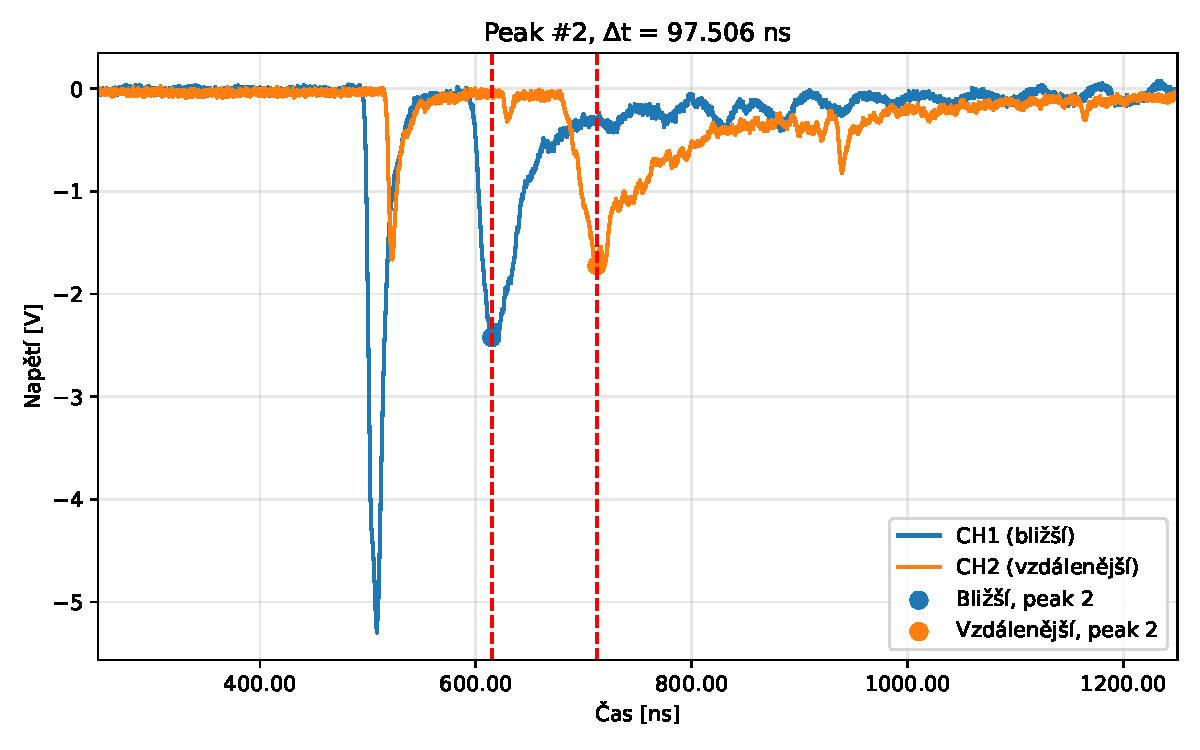
\includegraphics[width=0.90\textwidth]{img/charts/neutrony.pdf}
\caption{Detekované neutronové peaky z detektorů, měřeno při 7. výstřelu}
\label{fig:neutrony}
\end{figure}

Vypočtené $\Delta t$ se tedy rovná $97,506\ ns$, takže můžeme vypočítat energii jako:

$$
E_n = \frac{1}{2}m_n v^2 =  \frac{1}{2} 1,675 \times 10^{-27} \left(\frac{1,75}{97,506 \times 10^{-9} }\right)^2 = \boxed{1,68 \ \text{MeV}}
$$

U D-D neutronů bychom ale očekávali hodnotu okolo $2,54\ MeV$, naše je výrazně menší. To je pravděpodobně způsobeno posuvem neutronového peaku na bližším detektoru vlivem rozptylu na olověné desce. Zkusíme tedy zvolit jinší metodu měření. Spočítáme čas letu jen pomocí jednoho detektoru a srovnání téměř okamžitého peaku fotonů a neutronového peaku.

\begin{figure}[H]
\centering
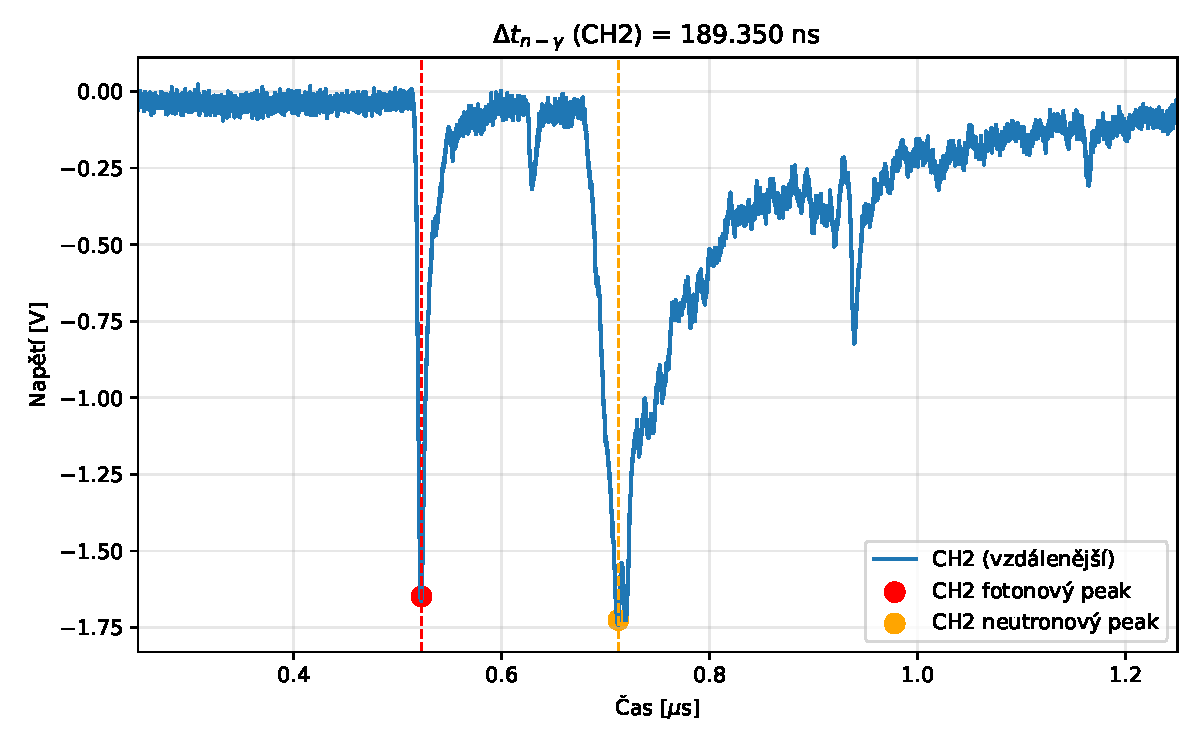
\includegraphics[width=0.90\textwidth]{img/charts/neutrony_better.pdf}
\caption{Detekované neutronové a fotonové peaky z detektorů, měřeno při 7. výstřelu}
\label{fig:neutrony}
\end{figure}

Podle následujícího vztahu a zjištěného $\Delta t_{n\gamma} = 189,350\ ns$ vypočítáme energii:
$$
\Delta t_{n\gamma} = t_n - t_\gamma \quad c = 2.998 \times 10^8\ \mathrm{m\,s^{-1}} \quad \frac{1}{c} = 3.33564\ \mathrm{ns\,m^{-1}}
$$

$$
t_{\mathrm{TOF}} = \Delta t_{n\gamma} + \frac{L}{c}
$$

$$
v_n = \frac{L}{t_{\mathrm{TOF}}} \quad E_n = \frac{1}{2} m_n v_n^2 \quad m_n = 1.675 \times 10^{-27}\ \mathrm{kg}
$$

$$
E_n =
5226
\left(
\frac{L[\mathrm{m}]}{t_{\mathrm{TOF}}[\mathrm{ns}]}
\right)^2
=
5226
\left(
\frac{4.25}{203.52}
\right)^2
=
\boxed{ 2.3\ \mathrm{MeV}}
$$


Vypočtená hodnota už je výrazně blíže k očekávané.


\section{Závěr}
Při experimentu na plazmatickém fokusu jsme pomocí scintilačních detektorů naměřili energii neutronů, které vznikají při fůzních reakcích uvnitř fokusovaného plazmatu. Určili jsme následující hodnotu:

$$
E_n = \boxed{2,3 \ \text{MeV}}
$$

\newpage
\section{Přílohy}
\begin{itemize}
    \item Python skript pro čtení detektorových dat a hledání peaků
    \item Data z osciloskopů a detektorů, rentgenové snímky plazmatu
\end{itemize}

\begin{thebibliography}{}

    \bibitem{zadani}
    Jakub Cikhardt, Pavel Kubeš. \textit{Prezentace k předmětu Fyzika pro elektroenergetiku}. 2025.

    \bibitem{skripta}
    Michal Bednařík. \textit{Studijní texty k předmětu Fyzika 2}.

\end{thebibliography}

\end{document}
